\svnid{$Id$}
\chapter{Nitrite Reduction in \Nm{}}
\label{chap:nitritereduction}

%In the case of this dataset, nitrite reduction has been modelled very well, but nitric oxide (and to a small extent, oxygen) has not been [Caveat, this may change when the cluster does eventually spit out the complete trajectory. This then could be moved into the discussion about why priors are important]. Not shown in Figure \ref{fig:no2sim} is the concentration of nitric oxide as nitrite is reduced. Unfortunately the parameter set used to generate the solved output assigned a very low value to the concentration of NorB (even though this should have been being expressed), thus the nitric oxide produced by reduction of nitrite does not itself get reduced, and towards the end of the dataset would be lethal to the culture. In this case, a different prior distribution should have been used for NorB concentration, as it was known beforehand that NorB concentration would be non-zero. This is an example of why the prior distributions are important.

\section{Microerobic Nitrite Reduction}
\subsection{Introduction}
\subsection{Results}
\subsection{Discussion}
\section{\texorpdfstring{Microaerobic Nitrite Reduction in \textit{norB$^\textrm{-}$} mutant}{Microaerobic Nitrite Reduction in norB- mutant}}
\subsection{Introduction}
\subsection{Results}
\subsection{Discussion}
\section{\texorpdfstring{Aerobic Nitrite Reduction in \textit{nsrR$^\textrm{-}$} mutant}{Aerobic Nitrite Reduction in nsrR- mutant}}
\subsection{Introduction}
\begin{figure}[tbp]
  \centering
    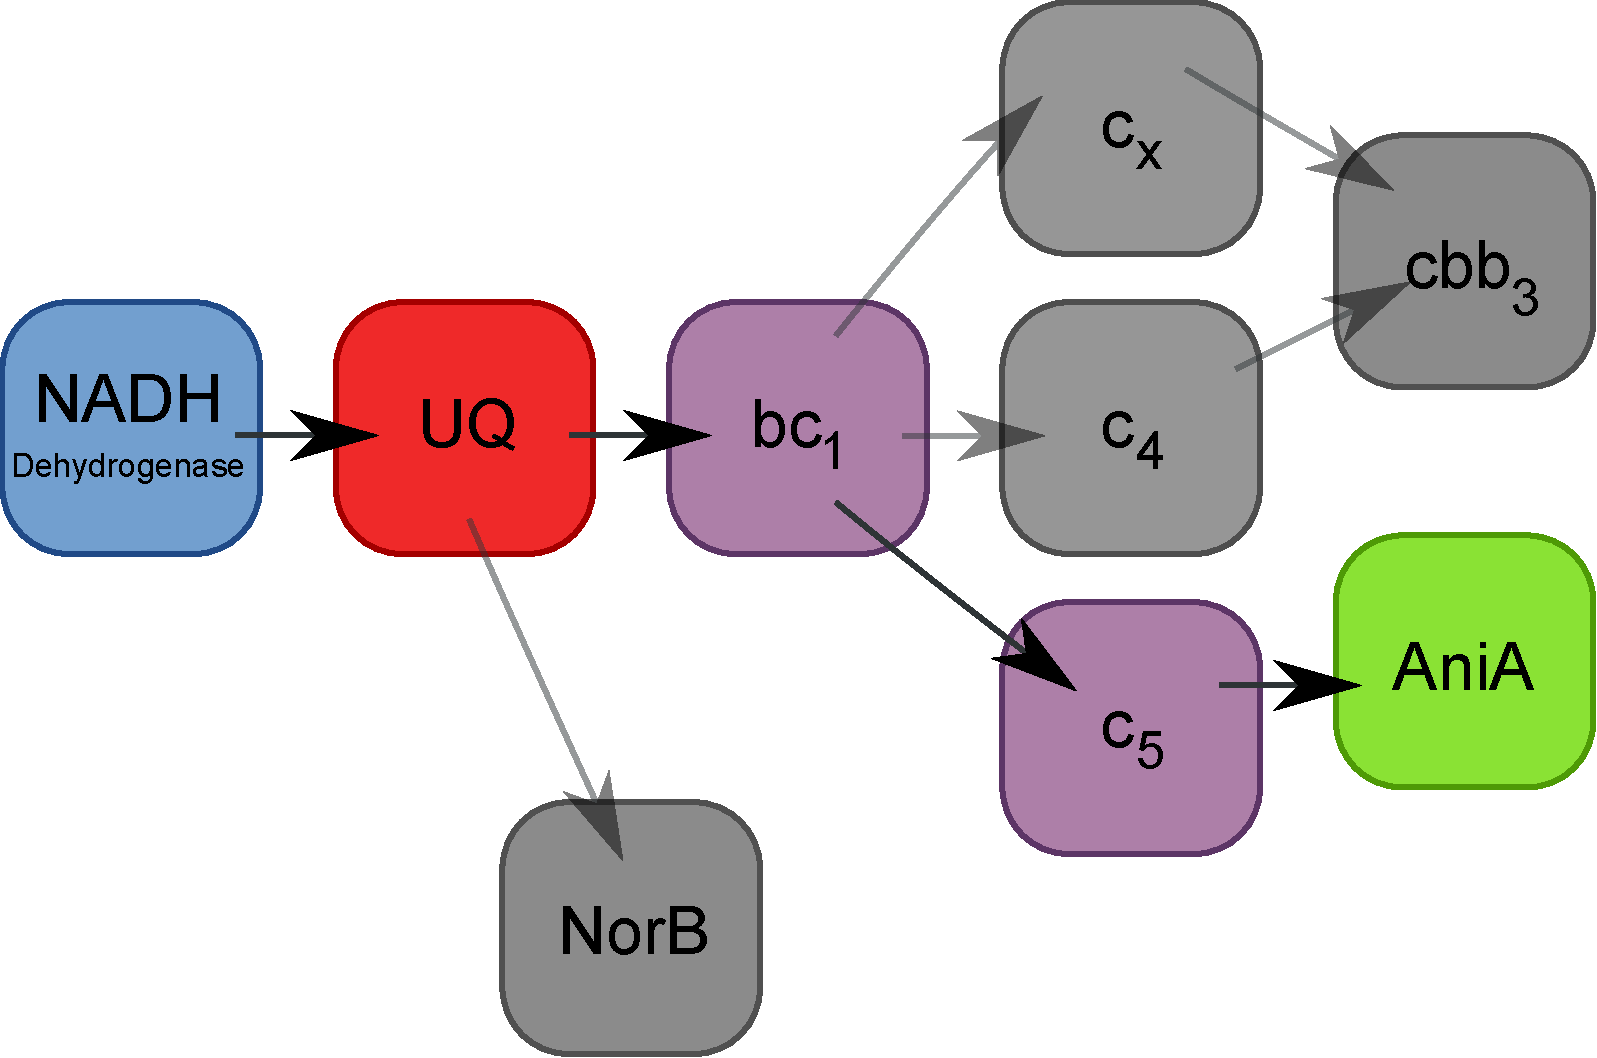
\includegraphics[width=14cm]{07-nitritereduction/data/no2_resp_chain.pdf}
    \caption[Nitrite reducing electron transport chain of \Nm{}]{{\bf Nitrite reducing electron transport chain of \Nm{}.} This shows the complete electron transport chain of \Nsm{} with the components irrelevant to nitrite reduction greyed out. In the mathematical model all of the purple elements (cytochromes) are amalgamated into one entity.
  \label{fig:no2_resp_chain}}
\end{figure}
Modelling nitrite reduction involves growing NsrR deficient cultures in aerobic conditions. This mutant expresses AniA and NorB in a constitutive manner, removing the necessity for growing the cultures in microaerobic conditions. The cultures are grown for 3-4 hours after which the culture is added to the electrode chamber and Sodium Nitrite added to a concentration of 1 mM.

In the model, Equations (\ref{eq:nitrite} \& \ref{eq:active_ania}) are now also involved, allowing parametrisation of kinetic rates of AniA. This experimental dataset does not unfortunately describe how the concentration of NO changes while Nitrite is being reduced. The prior probability distributions used for this dataset were the posteriors generated from the Nitric Oxide Reduction dataset described above, in accordance with Bayesian inference. The unknown parameters were given non-zero values with flat priors, allowed to burn-in and were then used to generate posterior probability distributions.

This is a simpler dataset than for Nitric oxide reduction as it only describes nitrite reduction, along with a small change in oxygen concentration. In combination with prior probability distributions from the afore mentioned dataset it means that the possible values for the kinetic rates involved are automatically going to be limited to those that work alongside the given priors. Without the prior probability distributions the posterior distributions would have a similar outcome to that of the first dataset used, where simple oxygen reduction was modelled, i.e. very wide distributions.
\subsection{Results}
\begin{figure}[tbp]
 \centering
 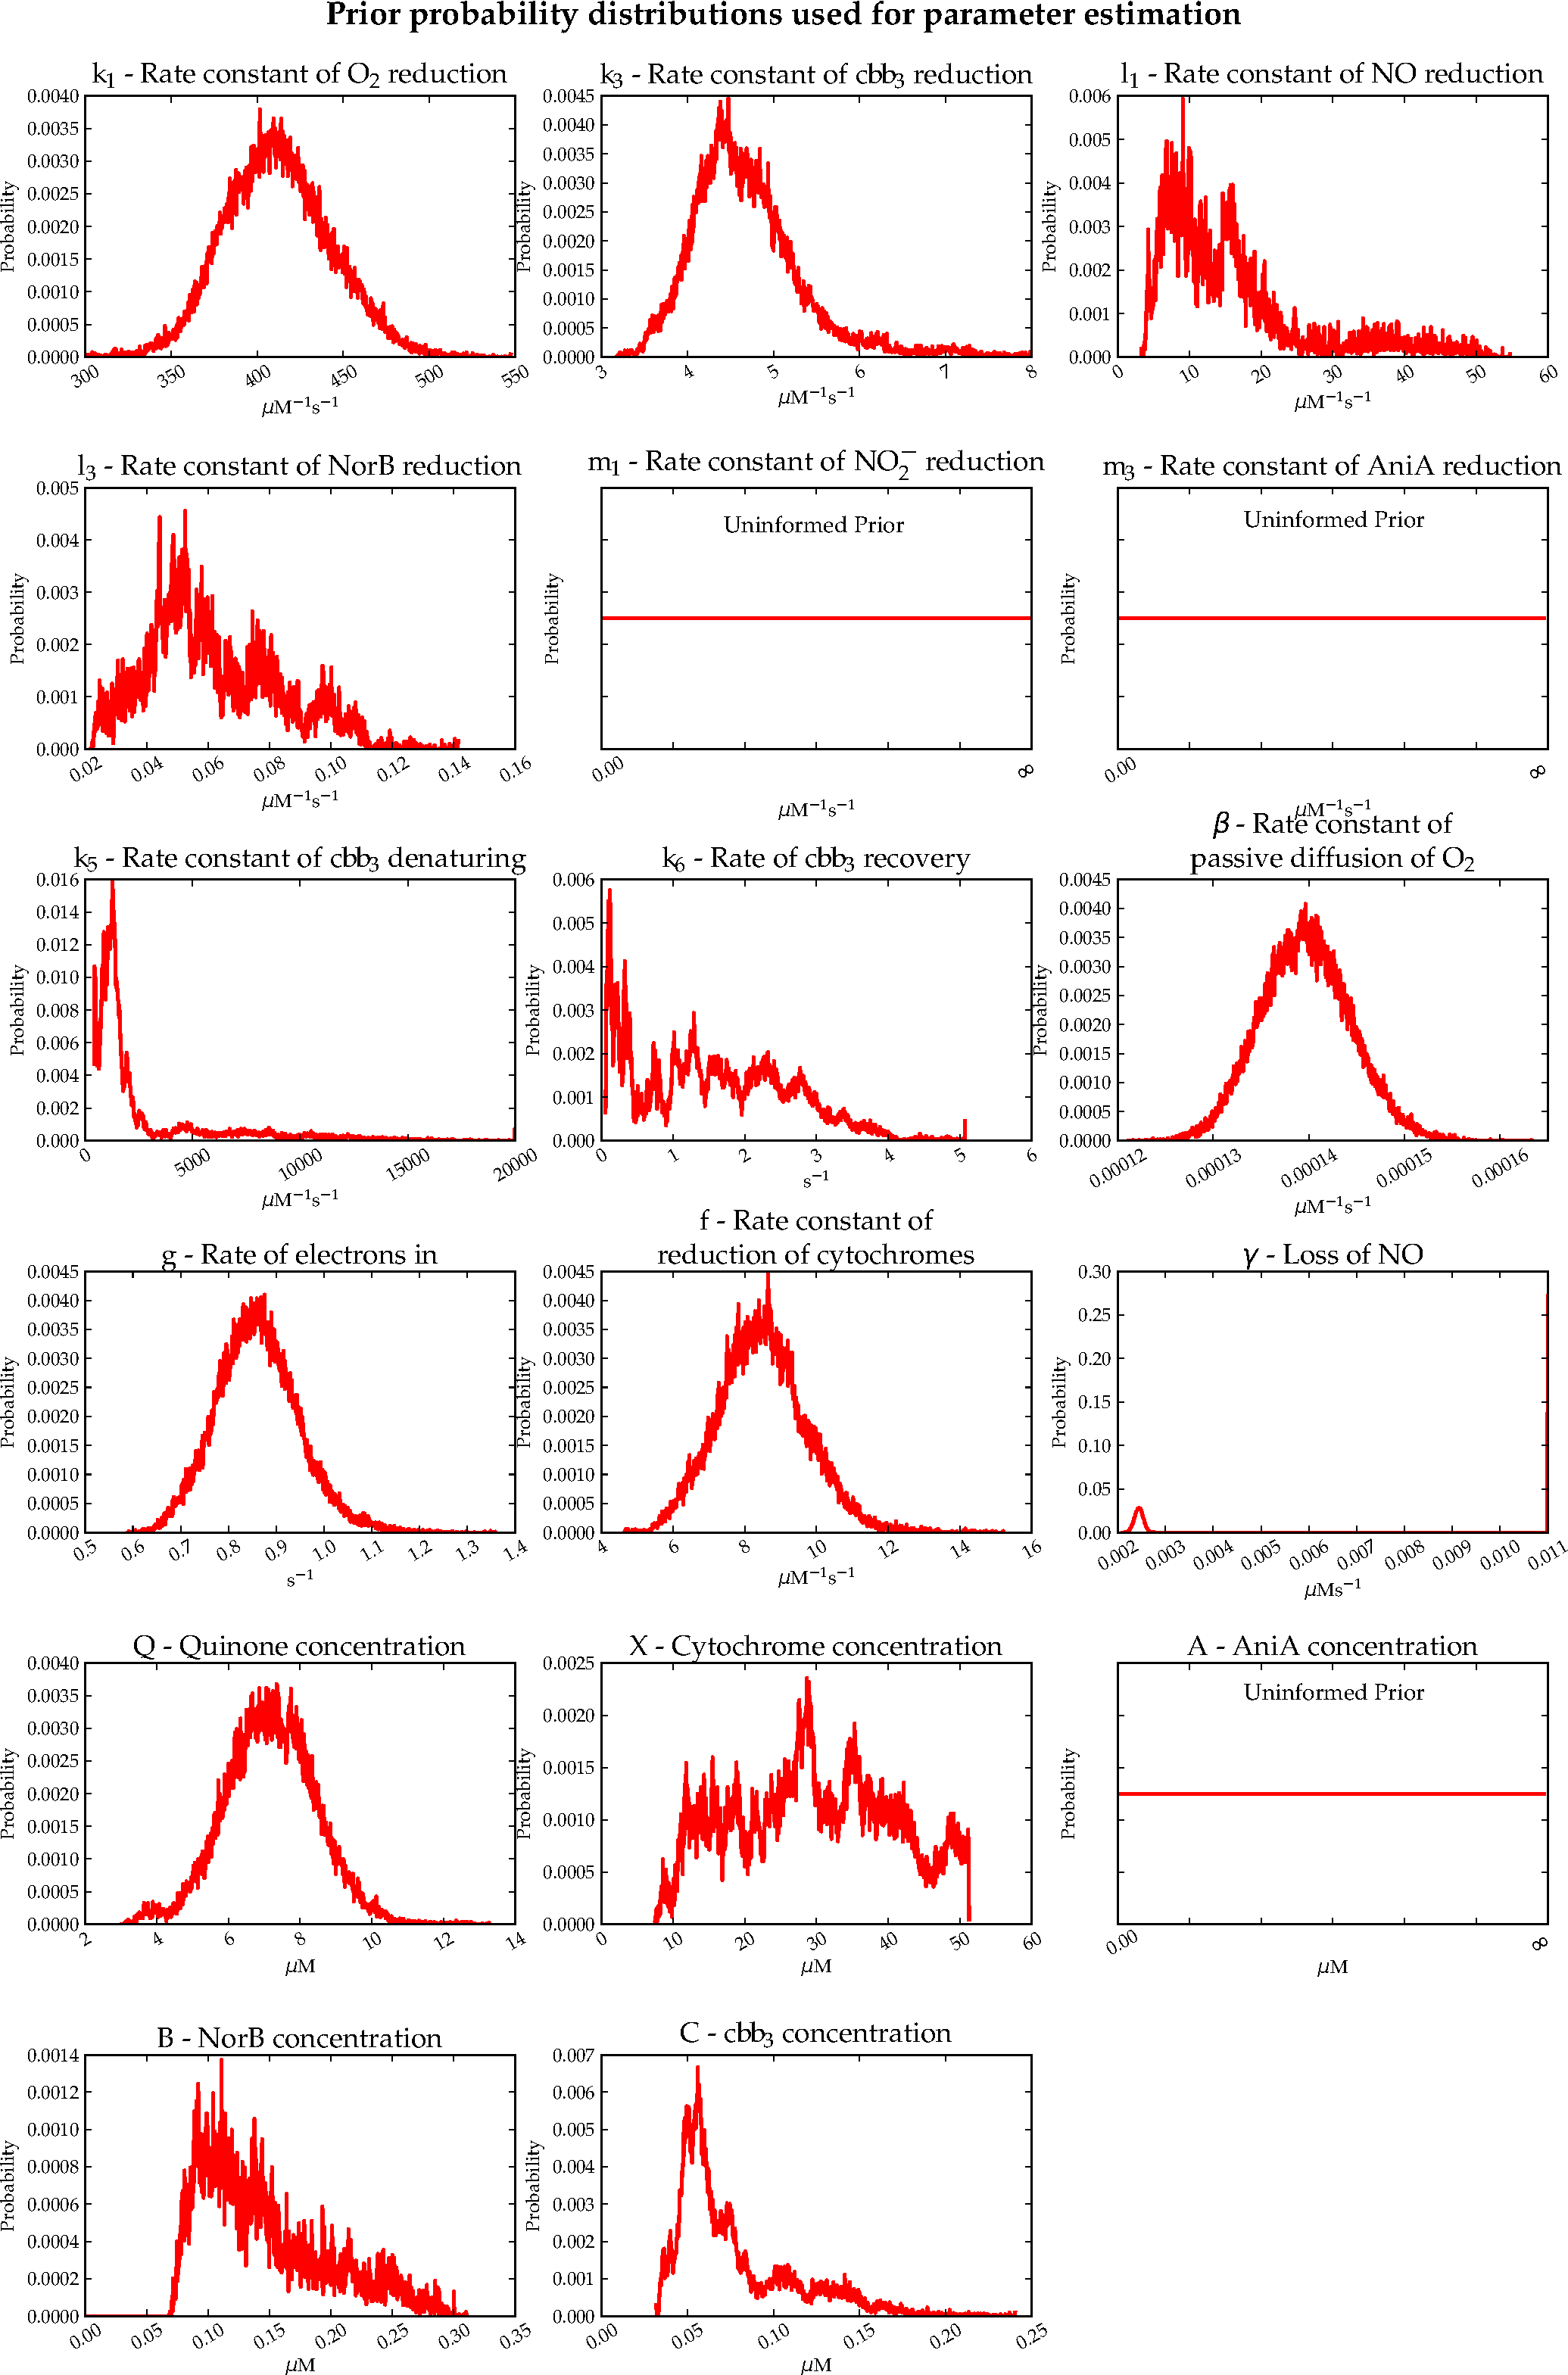
\includegraphics[width=15cm, trim=0cm 0cm 0cm 0cm]{./07-nitritereduction/data/priors1.pdf}
 % priors.pdf: 1008x1008 pixel, 72dpi, 35.56x35.56 cm, bb=0 0 1008 1008
 \caption[Prior probability distributions for microaerobic oxygen and nitrite reduction]{{\bf Prior probability distributions for microaerobic oxygen and nitrite reduction}. These are the probability distributions used as priors by the parameter estimation algorithm.
 \label{fig:nitrite_priors1}}
\end{figure}
\afterpage{\clearpage}





1st results on both datasets don't work very well. o2 reduction rate is too high on my data and norb is non-existent due to limitations in the experimental data, i.e. no fitting done to NO. NO doesn't increase when o2 reduction stops in rock data as it seems that g and f are too high causing X to be effectively permanently reduced. Unknown if NO2- data is correct due to same limitation as above. All 3 cannot reliably be determined at once.

Show all the results figures and the reduction state plots to corroborate.

Re-run simulations: my data broaden k1 and k3 and same for l1 l3 to try and fix both o2 reduction rate an no-non-reduction. C maybe needs to decrease. NO reduction rate should roughly equal O2 reduction rate (in denitrifying conditions) according to \citet{Rock2005}. Therefore l1*B should equal k1*C ish.
Rock data reset to zero and reduce f and g to try and get Q and X to be less reduced to trigger an increase in NO when O2 runs out. Q pool redox states differ (in paracoccus) \cite{Otten1999}.

Plot again with redox states to confirm or reject.

These changes will no doubt break the previous results (o2 and NO), but that is not necessarily a huge problem. The model seems capable of simulating the effect of nitric oxide on oxygen reduction rate, but in order to effect the changes in microaerobic conditions more drastic changes have to be made. This is quite likely as a result of the simplification of the redox chain in that all cytochromes are treated as one entity rather than the 4ish that actually exist. With all cytochromes modelled individually the potential redox state of bc1 could be different to that of cx,c4,c5 which could negate the need to alter f and g to lower the overall reduction state of X. If this is the case it goes a way to explain why the redox chain appears to be so complicated \textit{in vivo} rather than just have 1 serve-all cytochrome. Sadly this is something that was not possible to investigate in this study but could be included in further work onthe subject.

\subsection{Discussion}
\section{\texorpdfstring{Aerobic Nitrite Reduction in \textit{nsrR$^\textrm{-}$-norB$^\textrm{-}$} mutant}{Aerobic Nitrite Reduction in nsrR- - norB- mutant}}
\subsection{Introduction}
\subsection{Results}
\subsection{Discussion}